\documentclass{beamer}
%
% Choose how your presentation looks.
%
% For more themes, color themes and font themes, see:
% http://deic.uab.es/~iblanes/beamer_gallery/index_by_theme.html
%
\mode<presentation>
{
  \usetheme{Madrid}      % or try Darmstadt, Madrid, Warsaw, ...
  \usecolortheme{beaver} % or try albatross, beaver, crane, ...
  \usefonttheme{serif}  % or try serif, structurebold, ...
  \setbeamertemplate{navigation symbols}{}
  \setbeamertemplate{caption}[numbered]
} 

\usepackage[english]{babel}
\usepackage{kotex}
\usepackage{tikz}
%\usepackage[utf8x]{inputenc}

\title[3D 그래픽스 프로그래밍]{그래픽스 강의노트 02 - 컴퓨터 그래픽스란}
\author{강영민}
\institute{동명대학교}
\date{2015년 2학기}

\begin{document}

%%%%%%%%%%%%%%%%%%%%%%%%%%%%%%%%%%%%%%%%%%%%%%%%%%%%%%%%%
\begin{frame}
  \titlepage
\end{frame}

% Uncomment these lines for an automatically generated outline.
%\begin{frame}{Outline}
%  \tableofcontents
%\end{frame}


%%%%%%%%%%%%%%%%%%%%%%%%%%%%%%%%%%%%%%%%%%%%%%%%%%%%%%%%%
\begin{frame}{컴퓨터 그래픽스란}
\begin{itemize}
\item 컴퓨터 그래픽스 = 컴퓨터를 이용한 그래픽스
	\begin{itemize}
	\item 그래픽스의 어원은 그리기, 쓰기 등을 의미하는 그리스어  ‘$\gamma\rho\alpha\varphi\acute{\eta}$(graph\'{e})’
	\item 어떠한 표면에 시각적인 표현을 드러내는 것
	\item 컴퓨터 그래픽스는 컴퓨터를 활용하여 시각적으로 관찰할 수 있는 영상을 생성하는 것
	\end{itemize}
\item 그래픽스는 단순히 시각 정보 그 자체를 의미하는 것이 아니라, 이러한 시각 정보를 생성하는 것과 관련된 다양한 이론과 기술을 다루는 분야
\end{itemize}
\end{frame}
%%%%%%%%%%%%%%%%%%%%%%%%%%%%%%%%%%%%%%%%%%%%%%%%%%%%%%%%%

%%%%%%%%%%%%%%%%%%%%%%%%%%%%%%%%%%%%%%%%%%%%%%%%%%%%%%%%%
\begin{frame}{3차원 컴퓨터 그래픽스의 의미}

\begin{itemize}
\item 컴퓨터 그래픽스는 매우 다양한 의미를 가짐.
	\begin{itemize}
	\item 컴퓨터를 이용한 영상 데이터의 표현과 조작
	\item 영상을 생성하고 조작하기 위한 다양한 기술
	\item 시각적 콘텐츠를 디지털 기술로 합성/조작하는 방법을 연구하는 전산학 분야
	\end{itemize}
\end{itemize}

\begin{itemize}
\item 3차원 컴퓨터 그래픽스
	\begin{itemize}
	\item 3차원 기하(geometry) 객체 표현을 사용하는 그래픽스 분야
	\item 컴퓨터 게임이나 영화의 경우 결과 영상은 2차원 공간인 모니터나 스크린에 표현되지만, 이 영상을 얻기 위해 처리되는 데이터는 3차원 공간에서 정의되고 조작되므로 3차원 컴퓨터 그래픽스
	\item 컴퓨터 그래픽스의 세부 분야는 모델링(modeling), 애니메이션(animation), 렌더링(rendering)
	\end{itemize}
\end{itemize}

\end{frame}
%%%%%%%%%%%%%%%%%%%%%%%%%%%%%%%%%%%%%%%%%%%%%%%%%%%%%%%%%



%%%%%%%%%%%%%%%%%%%%%%%%%%%%%%%%%%%%%%%%%%%%%%%%%%%%%%%%%
\begin{frame}{모델링 modeling}

\begin{itemize}
\item 영상 생성에 사용되는 객체의 기하적 특성을 정의하는 일
	\begin{itemize}
	\item 객체를 표현하기 위해 사용되는 정점의 수를 결정
	\item 정점들의 위치와 연결성을 설정
	\item 그려질 면을 구성하는 일
	\end{itemize}
\end{itemize}
\end{frame}
%%%%%%%%%%%%%%%%%%%%%%%%%%%%%%%%%%%%%%%%%%%%%%%%%%%%%%%%%

%%%%%%%%%%%%%%%%%%%%%%%%%%%%%%%%%%%%%%%%%%%%%%%%%%%%%%%%%
\begin{frame}{애니메이션 animation}

\begin{itemize}
\item 모델링 과정을 통해 결정된 기하객체에 대해 시간에 따른 변화를 설정하는 작업
\item 일반적으로 이 변화의 대상은 기하객체의 위치
\item 시간이 흐름에 따라 객체가 움직이는 모습을 생성
\item 위치만이 애니메이션의 유일한 대상은 아니며, 시간에 따라 색상이 변하든가 물체에 적용된 텍스처(texture)가 변하는 등의 일도 모두 애니메이션
\end{itemize}

\end{frame}
%%%%%%%%%%%%%%%%%%%%%%%%%%%%%%%%%%%%%%%%%%%%%%%%%%%%%%%%%

%%%%%%%%%%%%%%%%%%%%%%%%%%%%%%%%%%%%%%%%%%%%%%%%%%%%%%%%%
\begin{frame}{렌더링 rendering}

\begin{itemize}
\item 모델링된 기하객체를 최종 관찰 표면에 그려내어 영상을 생성하는 분야
\item 조명 모델을 이용하여 표면의 색상 및 밝기 등을 결정
\item 결정된 색상을 2차원의 공간으로 투영하여 영상을 생성
\end{itemize}
\end{frame}
%%%%%%%%%%%%%%%%%%%%%%%%%%%%%%%%%%%%%%%%%%%%%%%%%%%%%%%%%

%%%%%%%%%%%%%%%%%%%%%%%%%%%%%%%%%%%%%%%%%%%%%%%%%%%%%%%%%
\begin{frame}{그래픽스의 응용 - 캐드(CAD)}

\begin{itemize}
\item 컴퓨터를 활용한 설계, 즉 ‘Computer-Aided Design’의 머릿글자
\item 건축, 제조 등 다양한 분야의 설계에 적용
\item 컴퓨터 기반 제조(Computer-Aided Manufacturing) 기술로 발전
\end{itemize}

\begin{figure}
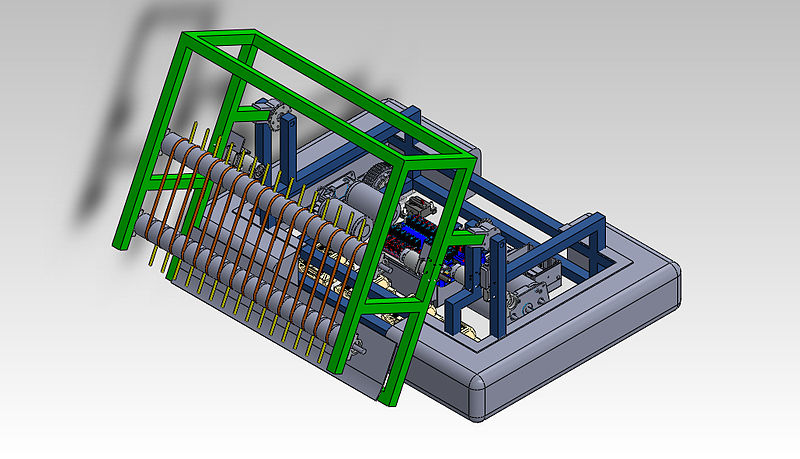
\includegraphics[width=11cm]{OGL_intro/CAD.jpg}
\end{figure}

\end{frame}
%%%%%%%%%%%%%%%%%%%%%%%%%%%%%%%%%%%%%%%%%%%%%%%%%%%%%%%%%


%%%%%%%%%%%%%%%%%%%%%%%%%%%%%%%%%%%%%%%%%%%%%%%%%%%%%%%%%
\begin{frame}{그래픽스의 응용 - 가상 현실(virtual reality)}

\begin{itemize}
\item 가상이라는 말은 ‘버추얼(virtual)’을 번역
\item ‘버추얼’이라는 단어는 ‘사실과 거의 차이가 없는’ 것의 의미
\item 가상현실을 가능하게 하는 기술적 요소는 입체화면, 3차원 입체 음향, 데이터 장갑 등의 입출력 장비,  컴퓨터 그래픽스 등
\item 실재감을 제공하기 위해 인지과학, 전자공학, 기계공학 등의 다양한 분야의 연구결과들을 적용
\end{itemize}

\begin{figure}
    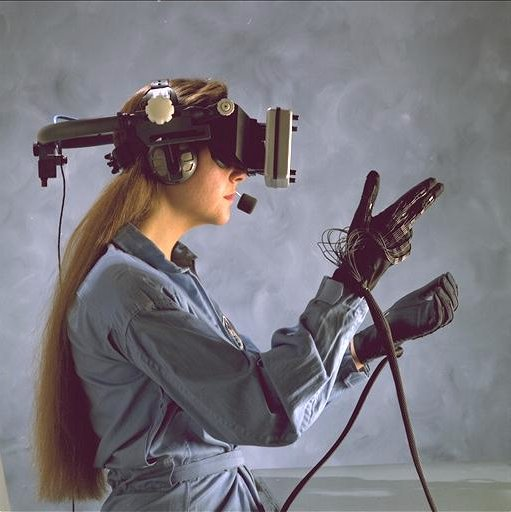
\includegraphics[width=4.5cm]{OGL_intro/virtualRealityHMD.jpg}
\end{figure}

\end{frame}
%%%%%%%%%%%%%%%%%%%%%%%%%%%%%%%%%%%%%%%%%%%%%%%%%%%%%%%%%

%%%%%%%%%%%%%%%%%%%%%%%%%%%%%%%%%%%%%%%%%%%%%%%%%%%%%%%%%
\begin{frame}{그래픽스의 응용 - 실사 수준 고품질 가시화}

\begin{itemize}
\item 가상 객체의 렌더링 결과를 실세계 물건과 구별이 어려워짐
\item 실사 수준의 고품질 가시화 기술이 다양한 산업 분야에 적용
\item 이미지를 얻는 데에 오랜 시간 소요 - 실시간 응용에 사용되지 않았음
\item 하드웨어 성능과 그래픽스 알고리즘 발전 - 실시간 응용에 점차 적용
\end{itemize}

\begin{figure}
    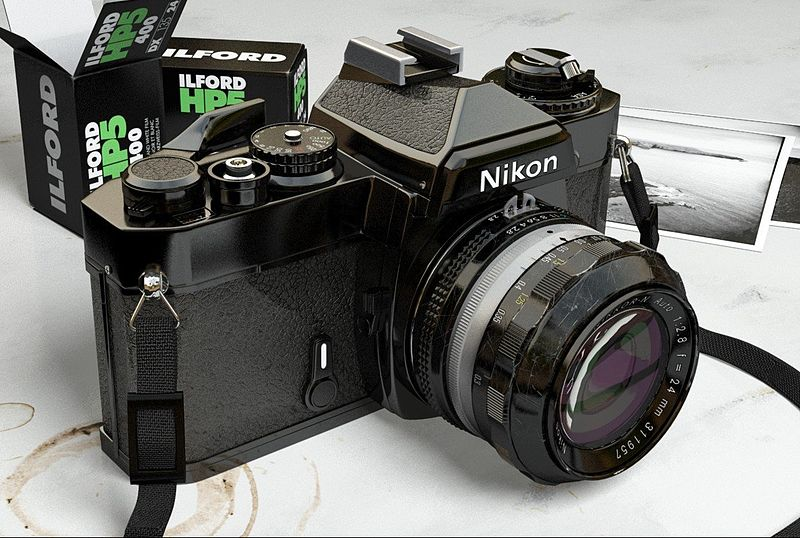
\includegraphics[width=7cm]{OGL_intro/photorealistic.jpg}
\end{figure}

\end{frame}
%%%%%%%%%%%%%%%%%%%%%%%%%%%%%%%%%%%%%%%%%%%%%%%%%%%%%%%%%

%%%%%%%%%%%%%%%%%%%%%%%%%%%%%%%%%%%%%%%%%%%%%%%%%%%%%%%%%
\begin{frame}{그래픽스의 응용 - 컴퓨터 아트(art)}

컴퓨터 그래픽스 기술은 예술적 창작물을 만드는 분야에도 다양하게 활용되고 있다. 

\begin{figure}
    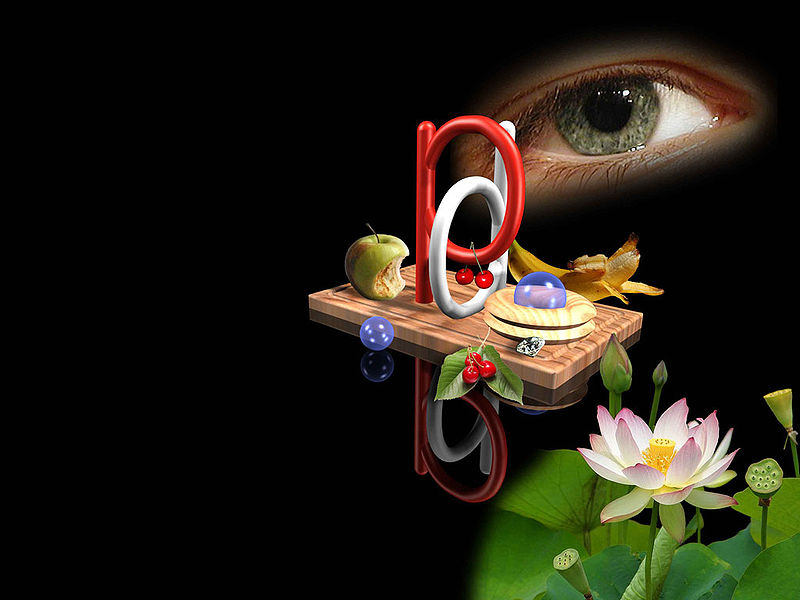
\includegraphics[width=9cm]{OGL_intro/computerArt.jpg}
\end{figure}

\end{frame}
%%%%%%%%%%%%%%%%%%%%%%%%%%%%%%%%%%%%%%%%%%%%%%%%%%%%%%%%%


%%%%%%%%%%%%%%%%%%%%%%%%%%%%%%%%%%%%%%%%%%%%%%%%%%%%%%%%%
\begin{frame}{그래픽스의 응용 - 컴퓨터 애니메이션/영화}

\begin{itemize}
\item 애니메이션/영화 산업에서 이제 컴퓨터 그래픽스는 가장 중요한 기술
\item 영화는 그 특성상 상호작용성(interactivity)이 요구되지 않음
\item 오랜 시간 동안 렌더링 작업을 수행하여 높은 수준의 영상 생성
\item 오프라인 렌더링(offline rendering)
\end{itemize}

\begin{figure}
\begin{tabular}{cc}
    
\includegraphics[height=4cm]{OGL_intro/animation.jpg}&
    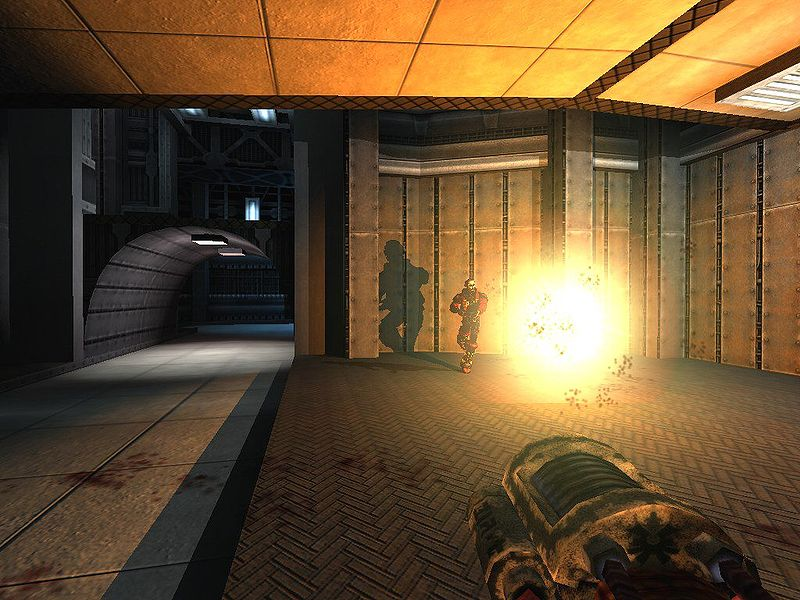
\includegraphics[height=4cm]{OGL_intro/game.jpg}\\
오프라인 렌더링 & 실시간 렌더링
\end{tabular}
\end{figure}


\end{frame}
%%%%%%%%%%%%%%%%%%%%%%%%%%%%%%%%%%%%%%%%%%%%%%%%%%%%%%%%%


%%%%%%%%%%%%%%%%%%%%%%%%%%%%%%%%%%%%%%%%%%%%%%%%%%%%%%%%%
\begin{frame}{그래픽스의 응용 - 컴퓨터 게임}

\begin{itemize}
\item 컴퓨터 그래픽스가 가장 상업적으로 성공한 분야 중에 하나
\item 상호작용성(interactivity)가 매우 중요
\item 실시간 고속 렌더링 기술이 매우 중요 - GPU 활용
\item 고품질의 영상을 빠른 시간에 그려내기 위한 다양한 기법을 발전
\end{itemize}

\begin{figure}
\begin{tabular}{cc}
    
\includegraphics[height=4cm]{OGL_intro/animation.jpg}&
    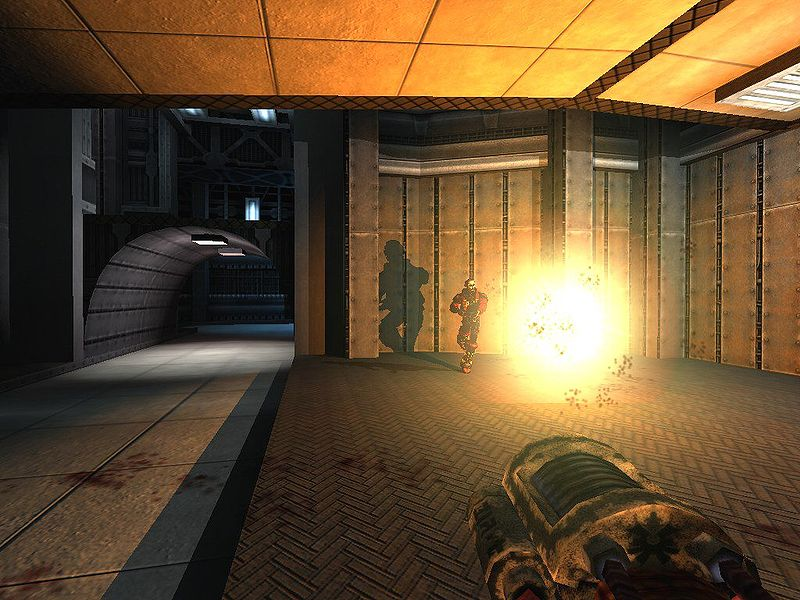
\includegraphics[height=4cm]{OGL_intro/game.jpg}\\
오프라인 렌더링 & 게임 그래픽스
\end{tabular}
\end{figure}

\end{frame}
%%%%%%%%%%%%%%%%%%%%%%%%%%%%%%%%%%%%%%%%%%%%%%%%%%%%%%%%%

%%%%%%%%%%%%%%%%%%%%%%%%%%%%%%%%%%%%%%%%%%%%%%%%%%%%%%%%%
\begin{frame}{그래픽스의 응용 - 교육 및 훈련}

\begin{itemize}
\item 강력한 가시화 기능은 교육과 훈련 분야에서 매우 효과적
\item 실제 환경에서 훈련하기 힘든 전투나, 항공기 조종 등의 훈련
\item 위험하거나 비용이 많이 드는 군사 분야 등에서 높은 활용도
\end{itemize}

\begin{figure}[h!]
  \centering
    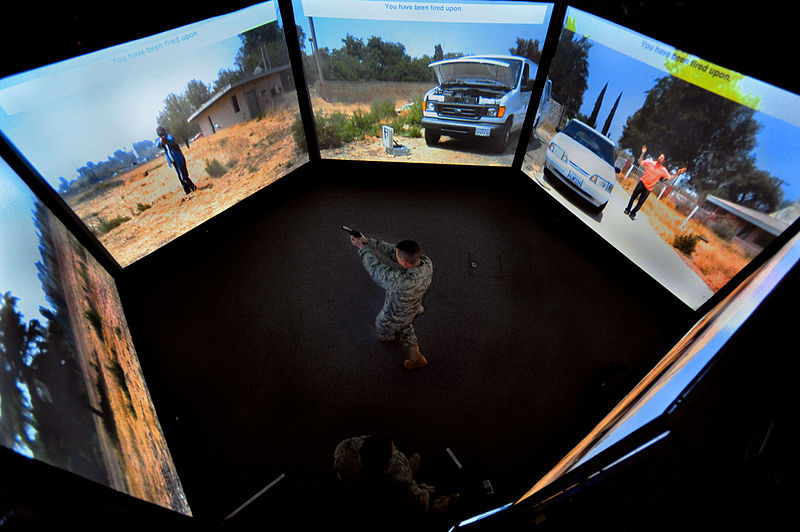
\includegraphics[height=4cm]{OGL_intro/virtualTraining.jpg}
    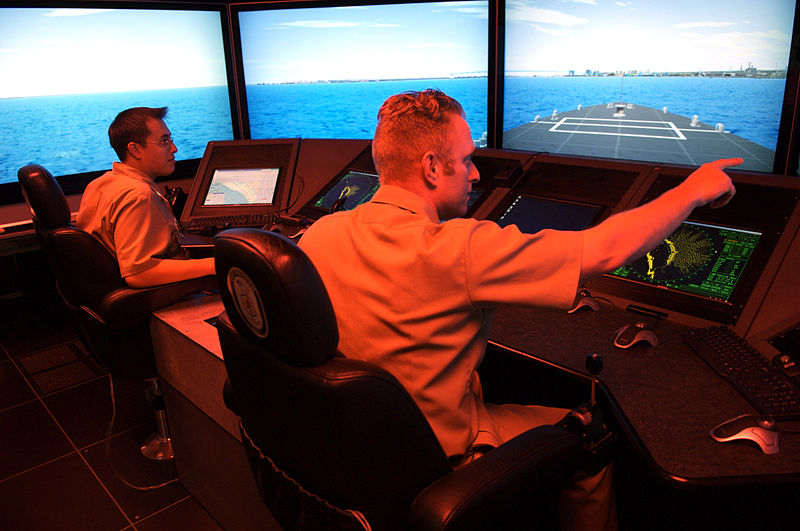
\includegraphics[height=4cm]{OGL_intro/virtualTraining2.jpg}
\end{figure}

\end{frame}
%%%%%%%%%%%%%%%%%%%%%%%%%%%%%%%%%%%%%%%%%%%%%%%%%%%%%%%%%

%%%%%%%%%%%%%%%%%%%%%%%%%%%%%%%%%%%%%%%%%%%%%%%%%%%%%%%%%
\begin{frame}{그래픽스의 응용 - 정보 가시화}

\begin{itemize}
\item 과학기술 분야에서 획득된 데이터를 이해하기 쉬운 형태로 표현
\item 자연 현상을 관찰하여 수집된 데이터
\item 계산을 통해 얻은 데이터
\item 현상을 직관적으로 이해할 수 있게 하며, 패턴이나 추세 등을 파악
\end{itemize}


\begin{figure}
    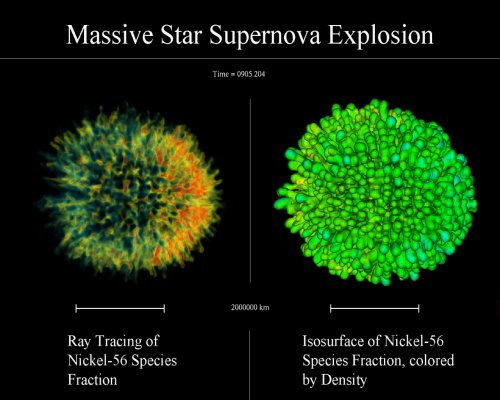
\includegraphics[height=5cm]{OGL_intro/visualization1.jpg}
    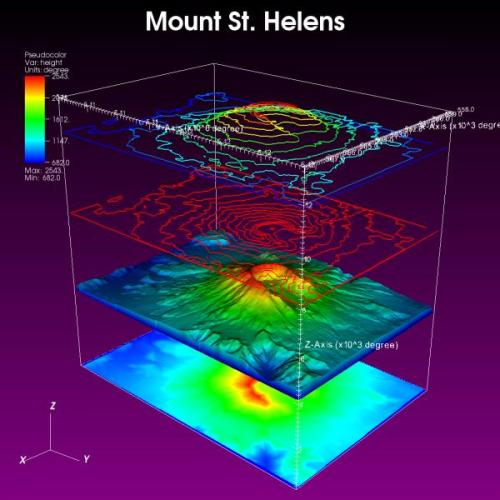
\includegraphics[height=5cm]{OGL_intro/visualization2.jpg}
\end{figure}

\end{frame}
%%%%%%%%%%%%%%%%%%%%%%%%%%%%%%%%%%%%%%%%%%%%%%%%%%%%%%%%%


%%%%%%%%%%%%%%%%%%%%%%%%%%%%%%%%%%%%%%%%%%%%%%%%%%%%%%%%%
\begin{frame}{그래픽스의 역사 - 1950년대}

\begin{itemize}
\item 컴퓨터 그래픽스가 시작된 시기
\item 컴퓨팅 역사의 초기
\item 래스터 장치 보다는 벡터 디스플레이 장치를 이용한 그래픽 표현
\item 초창기 게임이라고 할 수 있는 `테니스 포 투(Tennis for Two)'
\end{itemize}

\begin{figure}
    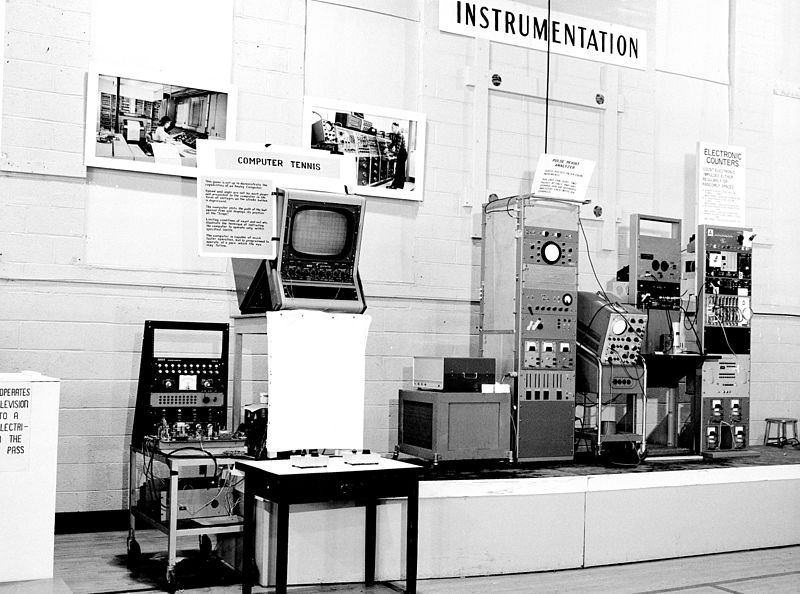
\includegraphics[height=5cm]{OGL_intro/tennis4two.jpg}
\end{figure}

\end{frame}
%%%%%%%%%%%%%%%%%%%%%%%%%%%%%%%%%%%%%%%%%%%%%%%%%%%%%%%%%

%%%%%%%%%%%%%%%%%%%%%%%%%%%%%%%%%%%%%%%%%%%%%%%%%%%%%%%%%
\begin{frame}{그래픽스의 역사 - 1960년대}

\begin{itemize}
\item 연결구조만을 가시화하는 와이어 프레임(wireframe) 가시화 수준
\item 다양한 그래픽 관련 기술과 산업이 출현
\item HMD(head mounted display) 장치도 이 무렵에 개발
\end{itemize}

\begin{figure}
    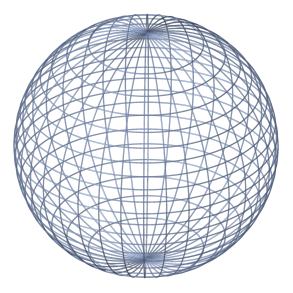
\includegraphics[height=6cm]{OGL_intro/wireframe.png}
\end{figure}

\end{frame}
%%%%%%%%%%%%%%%%%%%%%%%%%%%%%%%%%%%%%%%%%%%%%%%%%%%%%%%%%

%%%%%%%%%%%%%%%%%%%%%%%%%%%%%%%%%%%%%%%%%%%%%%%%%%%%%%%%%
\begin{frame}{그래픽스의 역사 - 1970년대}

\begin{itemize}
\item 래스터 그래픽스가 표준적인 그래픽스로 자리
\item 래스터 그래픽스는 벡터 그래픽스와 달리 면을 칠하는 것이 쉬움
\item 면의 음영을 결정하거나, 화소별 색상을 계산
\item 고품질 이미지 생성이 가능
\end{itemize}

\begin{figure}
    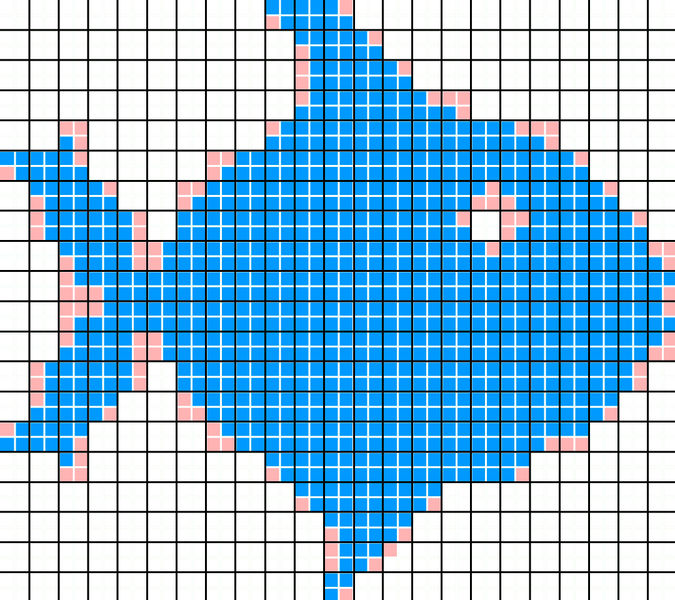
\includegraphics[height=4cm]{OGL_intro/rasterFish.jpg}
    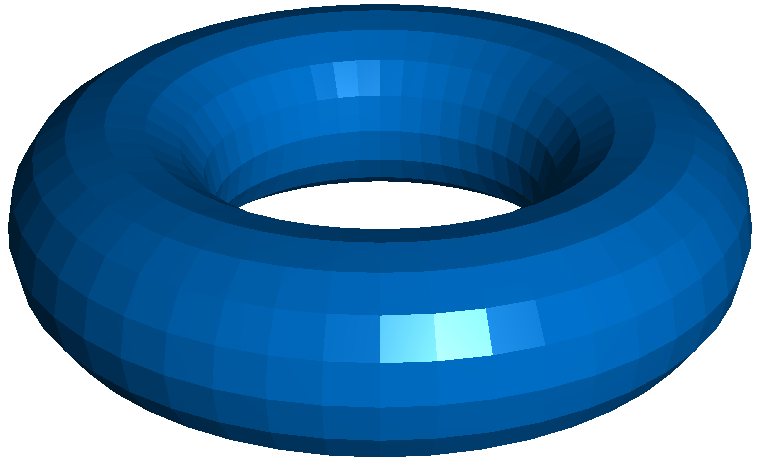
\includegraphics[height=4cm]{OGL_intro/flatShading.png}
\end{figure}

\end{frame}
%%%%%%%%%%%%%%%%%%%%%%%%%%%%%%%%%%%%%%%%%%%%%%%%%%%%%%%%%


%%%%%%%%%%%%%%%%%%%%%%%%%%%%%%%%%%%%%%%%%%%%%%%%%%%%%%%%%
\begin{frame}{그래픽스의 역사 - 1980년대}

\begin{itemize}
\item 그래픽스 관련 기술이 고도화
\item 개인용 컴퓨터 보급으로 제한된 자원을 활용한 기술 연구 활발
\item 고품질 이미지 생성 영역도 비약적인 발전
\item 컴퓨터의 성능이 비약적으로 발전 - 구현이 어려웠던 광선 추적법(ray tracing) 등의 기술을 활용한 이미지 생성
\end{itemize}

\begin{figure}
    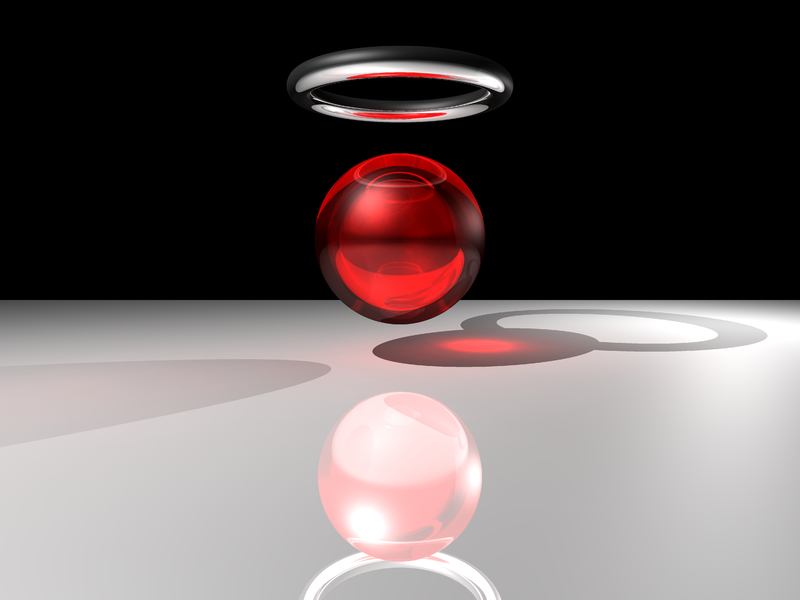
\includegraphics[width=7cm]{OGL_intro/raytracing.png}
\end{figure}

\end{frame}
%%%%%%%%%%%%%%%%%%%%%%%%%%%%%%%%%%%%%%%%%%%%%%%%%%%%%%%%%

%%%%%%%%%%%%%%%%%%%%%%%%%%%%%%%%%%%%%%%%%%%%%%%%%%%%%%%%%
\begin{frame}{그래픽스의 역사 - 1990년대}

\begin{itemize}
\item 그래픽스 처리 전담 하드웨어가 개인용 컴퓨터 설치
\item 실시간 그래픽스 분야가 획기적인 발전
\item OpenGL API(application programming interface)가 완성
\item 개인용 컴퓨터에서도 텍스처 매핑, 블렌딩(blending) 가능
\item 다양한 종류의 버퍼(buffer) 활용 기술
\item 애니메이션 작품들이 대단한 성공 - 관련 산업의 발전
\end{itemize}

\begin{figure}
    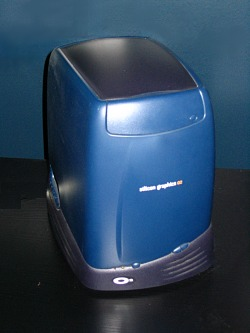
\includegraphics[height=4cm]{OGL_intro/SGI_O2.jpg}
    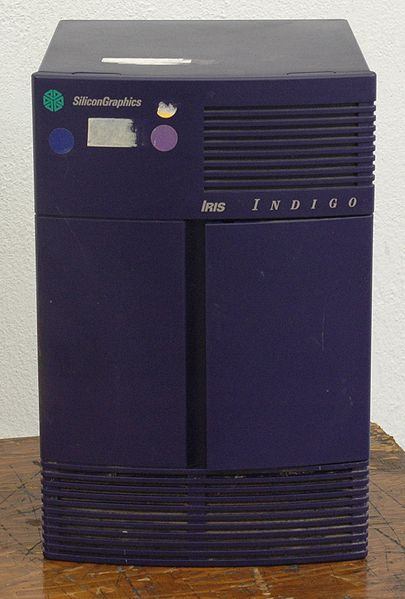
\includegraphics[height=4cm]{OGL_intro/SGI_Indigo.jpg}
    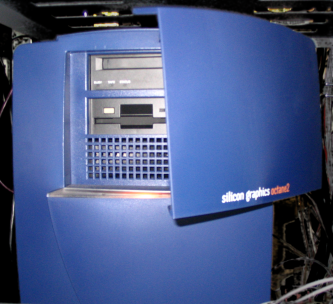
\includegraphics[height=4cm]{OGL_intro/SGI_Octane.png}
\end{figure}


\end{frame}
%%%%%%%%%%%%%%%%%%%%%%%%%%%%%%%%%%%%%%%%%%%%%%%%%%%%%%%%%

%%%%%%%%%%%%%%%%%%%%%%%%%%%%%%%%%%%%%%%%%%%%%%%%%%%%%%%%%
\begin{frame}{그래픽스의 역사 - 2000년대 이후}

\begin{itemize}
\item 극사실적 그래픽 표현 기술의 발전
\item 실시간 그래픽스 분야에서는 NVIDIA, ATI의 경쟁 구도
\item 게임이 시장의 중요한 동력
\item GPU의 병렬처리 능력을 활용
\end{itemize}

\begin{figure}
    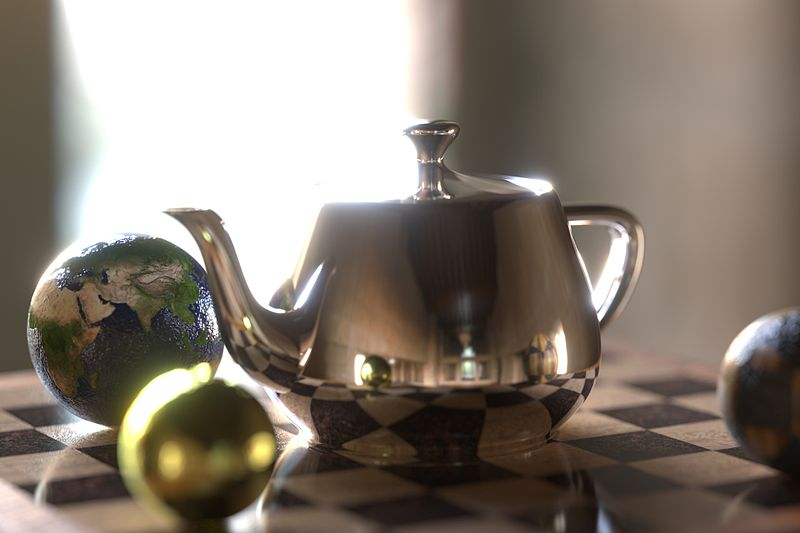
\includegraphics[width=8cm]{OGL_intro/photorealisticTeapot.jpg}
\end{figure}


\end{frame}
%%%%%%%%%%%%%%%%%%%%%%%%%%%%%%%%%%%%%%%%%%%%%%%%%%%%%%%%%


%%%%%%%%%%%%%%%%%%%%%%%%%%%%%%%%%%%%%%%%%%%%%%%%%%%%%%%%%
\begin{frame}{3차원 공간의 표현과 영상 생성의 기본 개념}

\begin{itemize}
\item 가상의 3차원 공간에 표현된 환경을 2차원 영상 이미지로 만들어 내는 일에는 기본적으로 다음과 같은 세 가지 물리적 요소가 고려되어야 함
	\begin{itemize}
	\item 광원(Light)
	\item 색(Color)
	\item 인지(Perception)
	\end{itemize}
\end{itemize}

\begin{itemize}
\item 합성 카메라 모델(synthetic camera model)
	\begin{itemize}
	\item 광학 시스템에서 영상이 맺히는 방식을 흉내내어 가상의 카메라를 만드는 것
	\item 객체, 관측자, 광원
	\end{itemize}
\end{itemize}	

\end{frame}
%%%%%%%%%%%%%%%%%%%%%%%%%%%%%%%%%%%%%%%%%%%%%%%%%%%%%%%%%


%%%%%%%%%%%%%%%%%%%%%%%%%%%%%%%%%%%%%%%%%%%%%%%%%%%%%%%%%
\begin{frame}{광원(Light Source)}

\begin{itemize}
\item 광원은 빛을 발생시키는 객체, 혹은 지점
\item 빛이란 전자기파의 일부로 우리 눈이 반응하는 스펙트럼 영역
\item 390nm~720nm 정도의 범위의 전자기파
\item 파장인 긴 쪽은 붉은색 짧은 쪽은 자색
\item 광원이 중요한 이유는 우리가 영상으로 담아내는 내용은 빛이 객체와 반응하여 관측자에게 도달한 결과이기 때문
\end{itemize}

\end{frame}
%%%%%%%%%%%%%%%%%%%%%%%%%%%%%%%%%%%%%%%%%%%%%%%%%%%%%%%%%


%%%%%%%%%%%%%%%%%%%%%%%%%%%%%%%%%%%%%%%%%%%%%%%%%%%%%%%%%
\begin{frame}{광선 추적 기법(Ray Tracing Method)}

\begin{itemize}
\item 영상이 빛을 담아내는가장 간단한 접근법은 광원에서 나온 빛을 추적하여 객체에 충돌하고 반사하는 과정을 계산한 뒤에 관측자의 영상 시스템에 도달하는 결과를 알아내는 것
\item 이 방법의 단점은 빛과 객체의 상호작용을 완벽히 추적하는 것이 불가능하다는 점
\end{itemize}

\begin{figure}
    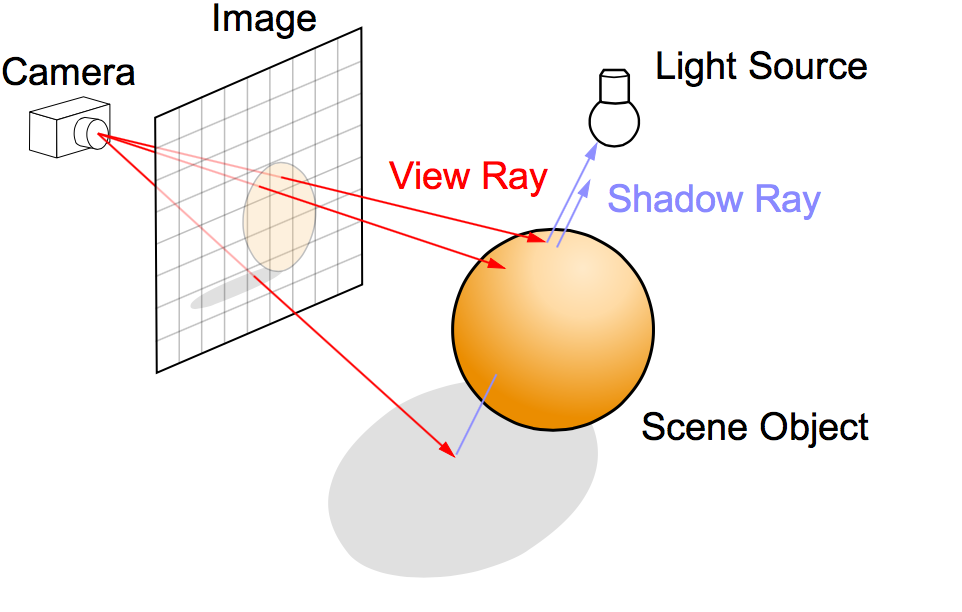
\includegraphics[height=5cm]{OGL_intro/raytracingConcept.png}
\end{figure}

\end{frame}
%%%%%%%%%%%%%%%%%%%%%%%%%%%%%%%%%%%%%%%%%%%%%%%%%%%%%%%%%

%%%%%%%%%%%%%%%%%%%%%%%%%%%%%%%%%%%%%%%%%%%%%%%%%%%%%%%%%
\begin{frame}{바늘구멍 카메라(Pinhole Camera)}

\begin{itemize}
\item 구멍을 통해 들어온 빛이 반대편 벽에 상을 맺게 함
\item 상의 위치 $(x_p, y_p, z_p)$는 간단한 원근 투영법으로 계산 가능
\end{itemize}



\begin{eqnarray}
\left ( x_p = - \frac{x d}{z} , y_p = - \frac{yd}{z}, z_p = -d \right )
\end{eqnarray}

\begin{figure}[h!]
  \centering
    \begin{tikzpicture} [scale=3]
      \draw  (0,0) -- (1,0) -- (1,0.5) -- (0,0.5) -- cycle;
	\draw (0.5, 0.25) -- (1.5, 0.25) -- (1.5, 0.75) -- (0.5, 0.75) -- cycle;
	\draw (0.5, 0.75) -- (0,0.5);
	\draw (0.5, 0.25) -- (0,0);
	\draw (1.5,0.75) -- (1.0,0.5);
	\draw (1.5, 0.25) -- (1.0,0);
	\draw [<->] (0,-0.25) -- (1,-0.25);
	\draw (0.5,-0.3) node {$d$};
	\draw (1.25, 0.375) circle (0.04);
	\draw [->] (1.25, 0.375) -- (2.0, 0.375);
	\draw [->] (1.25, 0.375) -- (1.25, 1.0);
	\draw [->] (1.25, 0.375) -- (1.75, 0.65);
	\draw (0.20, 0.17) -- (1.75, 0.5);
	\draw [fill] (0.2,0.17) circle [radius=0.02];
	\draw [fill] (1.75,0.5) circle [radius=0.02];
	\draw (0.0, 0.27) node (xp) {$(x_p, y_p, z_p)$};
	\draw (2.0, 0.5) node (xp) {$(x, y, z)$};
	\draw (2.0, 0.3) node {$x$};
	\draw (1.4, 1.0) node {$y$};
	\draw (1.75, 0.75) node {$z$};
   \end{tikzpicture}
\end{figure}

\end{frame}
%%%%%%%%%%%%%%%%%%%%%%%%%%%%%%%%%%%%%%%%%%%%%%%%%%%%%%%%%

%%%%%%%%%%%%%%%%%%%%%%%%%%%%%%%%%%%%%%%%%%%%%%%%%%%%%%%%%
\begin{frame}{합성 카메라 모델}

\begin{itemize}
\item 가상의 광학 시스템을 구성하여 가상 객체를 담아내는 것
\item 구멍을 통과하기 전에 적절한 거리 d 만큼 앞에 구멍을 향해 진행하는 빛을 잡아낼 수 있는 평면
\item 상이 거꾸로 맺히는 것과 달리 원래의 모양대로 상이 맺힘
\item 상이 맺히는 곳은 다음과 같이 계산할 수 있다.
\end{itemize}


\begin{eqnarray}
\left ( x_p = \frac{x d}{z} , y_p = \frac{yd}{z}, z_p = d \right )
\end{eqnarray}

이러한 합성 카메라 모델은 객체와 관측자, 광원을 분리하여 다룰 수 있게 하며, 객체, 광원, 카메라의 속성을 설정하는 간단한 소프트웨어 API로 모델을 만들 수 있다. 또한 이 방식은 고속으로 처리가능한 하드웨어 구현이 용이하다는 장점도 가진다.
\end{frame}
%%%%%%%%%%%%%%%%%%%%%%%%%%%%%%%%%%%%%%%%%%%%%%%%%%%%%%%%%


%%%%%%%%%%%%%%%%%%%%%%%%%%%%%%%%%%%%%%%%%%%%%%%%%%%%%%%%%
\begin{frame}{전역 조명과 지역 조명}

\begin{figure}
	\begin{tabular}{cc}
	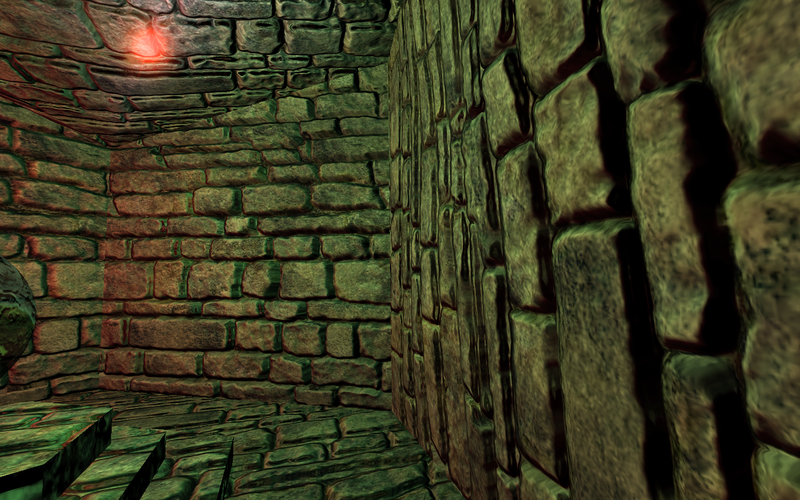
\includegraphics[height=4cm]{OGL_intro/realtimeEx.png} &    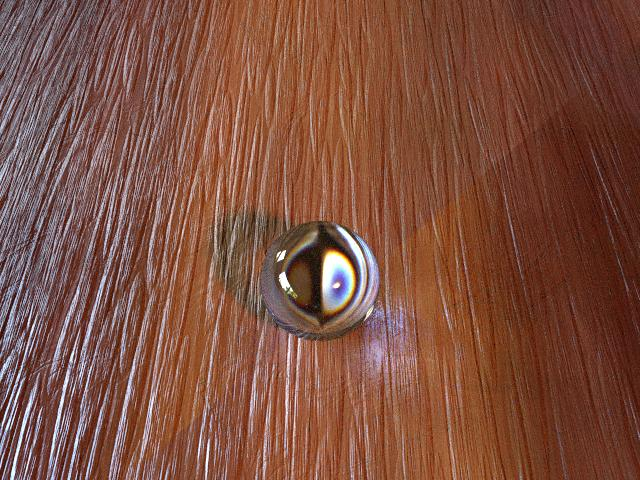
\includegraphics[height=4cm]{OGL_intro/offlineEx.jpg} \\
	(a) 지역조명 & (b) 전역조명
	\end{tabular}
\end{figure}

\end{frame}
%%%%%%%%%%%%%%%%%%%%%%%%%%%%%%%%%%%%%%%%%%%%%%%%%%%%%%%%%


\end{document}


